\begin{figure*}[htb]
\centering
\begin{minipage}{\fullwidthcaption}
\centering
\small
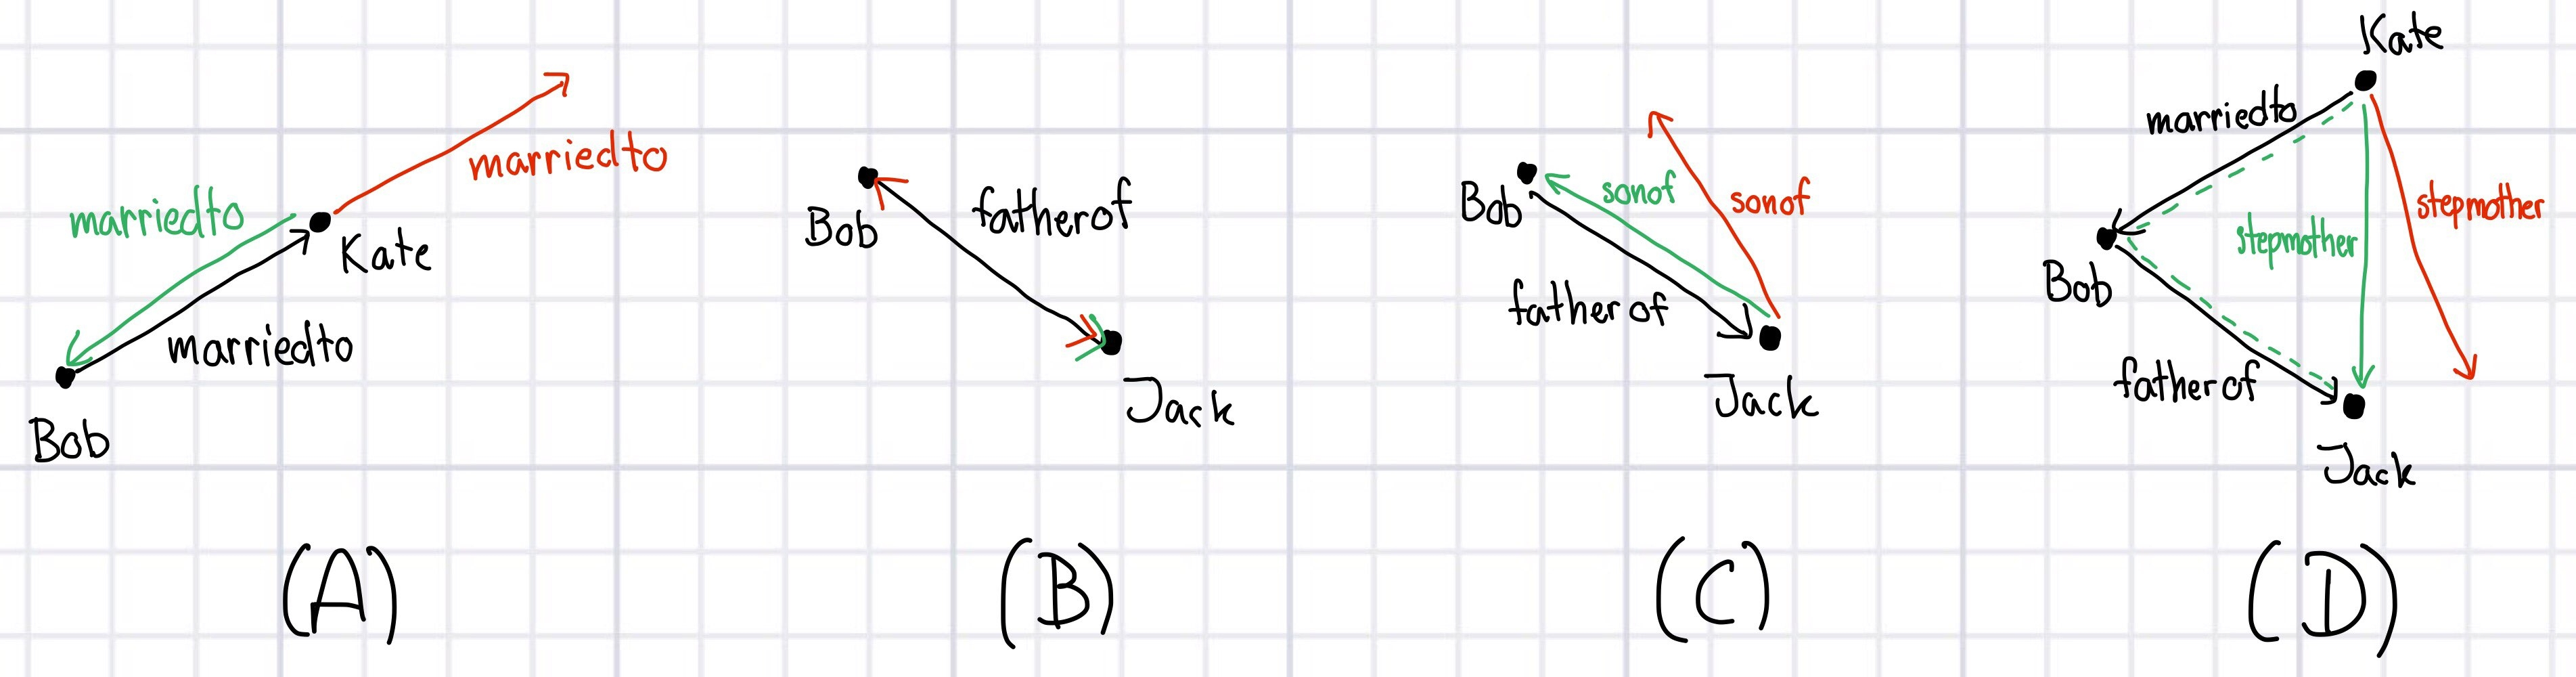
\includegraphics[scale=0.12]{content/hypotheses/figures/relation_properties_A-D.jpg}
\caption{Illustration of \autoref{hyp:relation_properties} A-D. Black is embedded information and red/green are different versions of the same relation embedding. Green is what the embedding should look like if the method can model relations with that property and red is what the embedding might look like if not. A: Symmetry, B: Anti-Symmtery, C: Inversion, D: Composition.
}
\label{fig:relation_properties_nothierarchy}
\end{minipage}
\end{figure*}